% !TeX TXS-program:compile = txs:///pdflatex/[--shell-escape]
% Le truc au-dessus pour avoir l'option shell-escape qui permet de faire du minted.
\documentclass[12pt]{article}

% Affichage ou non des reponses aux questions & exercices
\newif\ifDispRep
\DispReptrue  % Show the text
%\DispRepfalse % Hide the text

% Version du document
\newcommand{\versiondoc}{v0.1}

% Incorporation tous éléments de préambule communs à tous mes cours
% Sans chemin relatif parce que TexStudio lancé depuis un script qui prend en compte la variable d'environnement TEXINPUTS
\usepackage{CoursLFC}

% Eléments de l'en-tête et de la page de garde spécifiques à ce doc
\newcommand{\classe}{1\textsuperscript{ère} NSI}
\newcommand{\themecours}{Thème 7: Architecture Système}
\newcommand{\datedoc}{avril 2024}

% Page de garde mise en page
\title
	{\vspace{3cm}
		{\Large
		\textit
			{
				\classe\hspace{0.1cm}
				\textemdash\
				\hspace{0.1cm}
				\themecours
			}
			
		\vspace{1cm}
		\huge{Systèmes d'Exploitation \& Réseau} }
		 
		\vspace{1cm}
	}
\author{\etablissement}
\date{
	\auteur,
	\datedoc,
	\footnotesize{\textit{\versiondoc}} 
	\vspace{2cm}
	}

% Header & Footer
\lfoot{\etabshort}
\cfoot{\thepage}
\rfoot{\classe, \anneescol}
\renewcommand{\footrulewidth}{0.2pt}
\lhead{}
\chead{}
\rhead{}
\renewcommand{\headrulewidth}{0pt}

\begin{document}
	
	\maketitle
	% pas de footer sur la première page
	\thispagestyle{empty}
		
	\section*{}
		{\noindent
		\resumecours
		}
	
	\vspace{2cm}
	\begin{MaReponse}
		\centering
		\vspace{\baselineskip}
		\textbf{Document de cours incluant les réponses aux exercices.}
		\vspace{\baselineskip}
	\end{MaReponse}
		
	\pagebreak	
	\tableofcontents
	
	\pagebreak
	
	% Début du contenu du document

	\section{Point d'étape -- où est-on / où va-t-on?}
	\subsection{Ce qu'on a couvert jusqu'à présent}
	
	\begin{itemize}
		\item Rudiments de l'architecture physique d'un ordinateur -- le modèle de Von Neumann.
		\item Mise en jambes sur de l'écriture de code: réalisation d'une page Web en HTML.
		\item Introduction à Python, et plus spécifiquement:
		\begin{itemize}
			\item Ce qu'on appelle ses "constructions élémentaires" -- variables, fonctions, conditions \& embranchements, boucles...
			\item Les types et valeurs de base: entiers (naturels et relatifs), flottants (réels), chaînes de caractères et booléens (qu'on n'a que brièvement abordés pour l'instant).
			\item Un type dit "construit" -- les listes.
		\end{itemize}
		\item Un peu de théorie: la représentation des types et valeurs de base en machine (les entiers naturels et relatifs, les réels, les alphanumériques).
		\item Un peu plus de théorie: introduction à la logique booléenne (que l'on n'a couverte que très rapidement -- on y reviendra en fin d'année).
		\item Un retour à la pratique: le traitement de données en table, la manipulation de fichiers dans Python, et des types de données plus complexes --- les dictionnaires, les listes de dictionnaires...
		\item Une introduction à l'algorithmique, avec des allers-retours entre théorie et pratique: étude des principes d'algorithmes, rédaction de leur pseudo-code, implémentation en Python.
	\end{itemize}
	
	\subsection{Ce dont on va parler dans ce nouveau chapitre}
	
	On va revenir ici au tout premier cours qu'on a fait cette année, le modèle de von Neumann, et "remonter" de là:
	\begin{figure}[H]
		\centering
		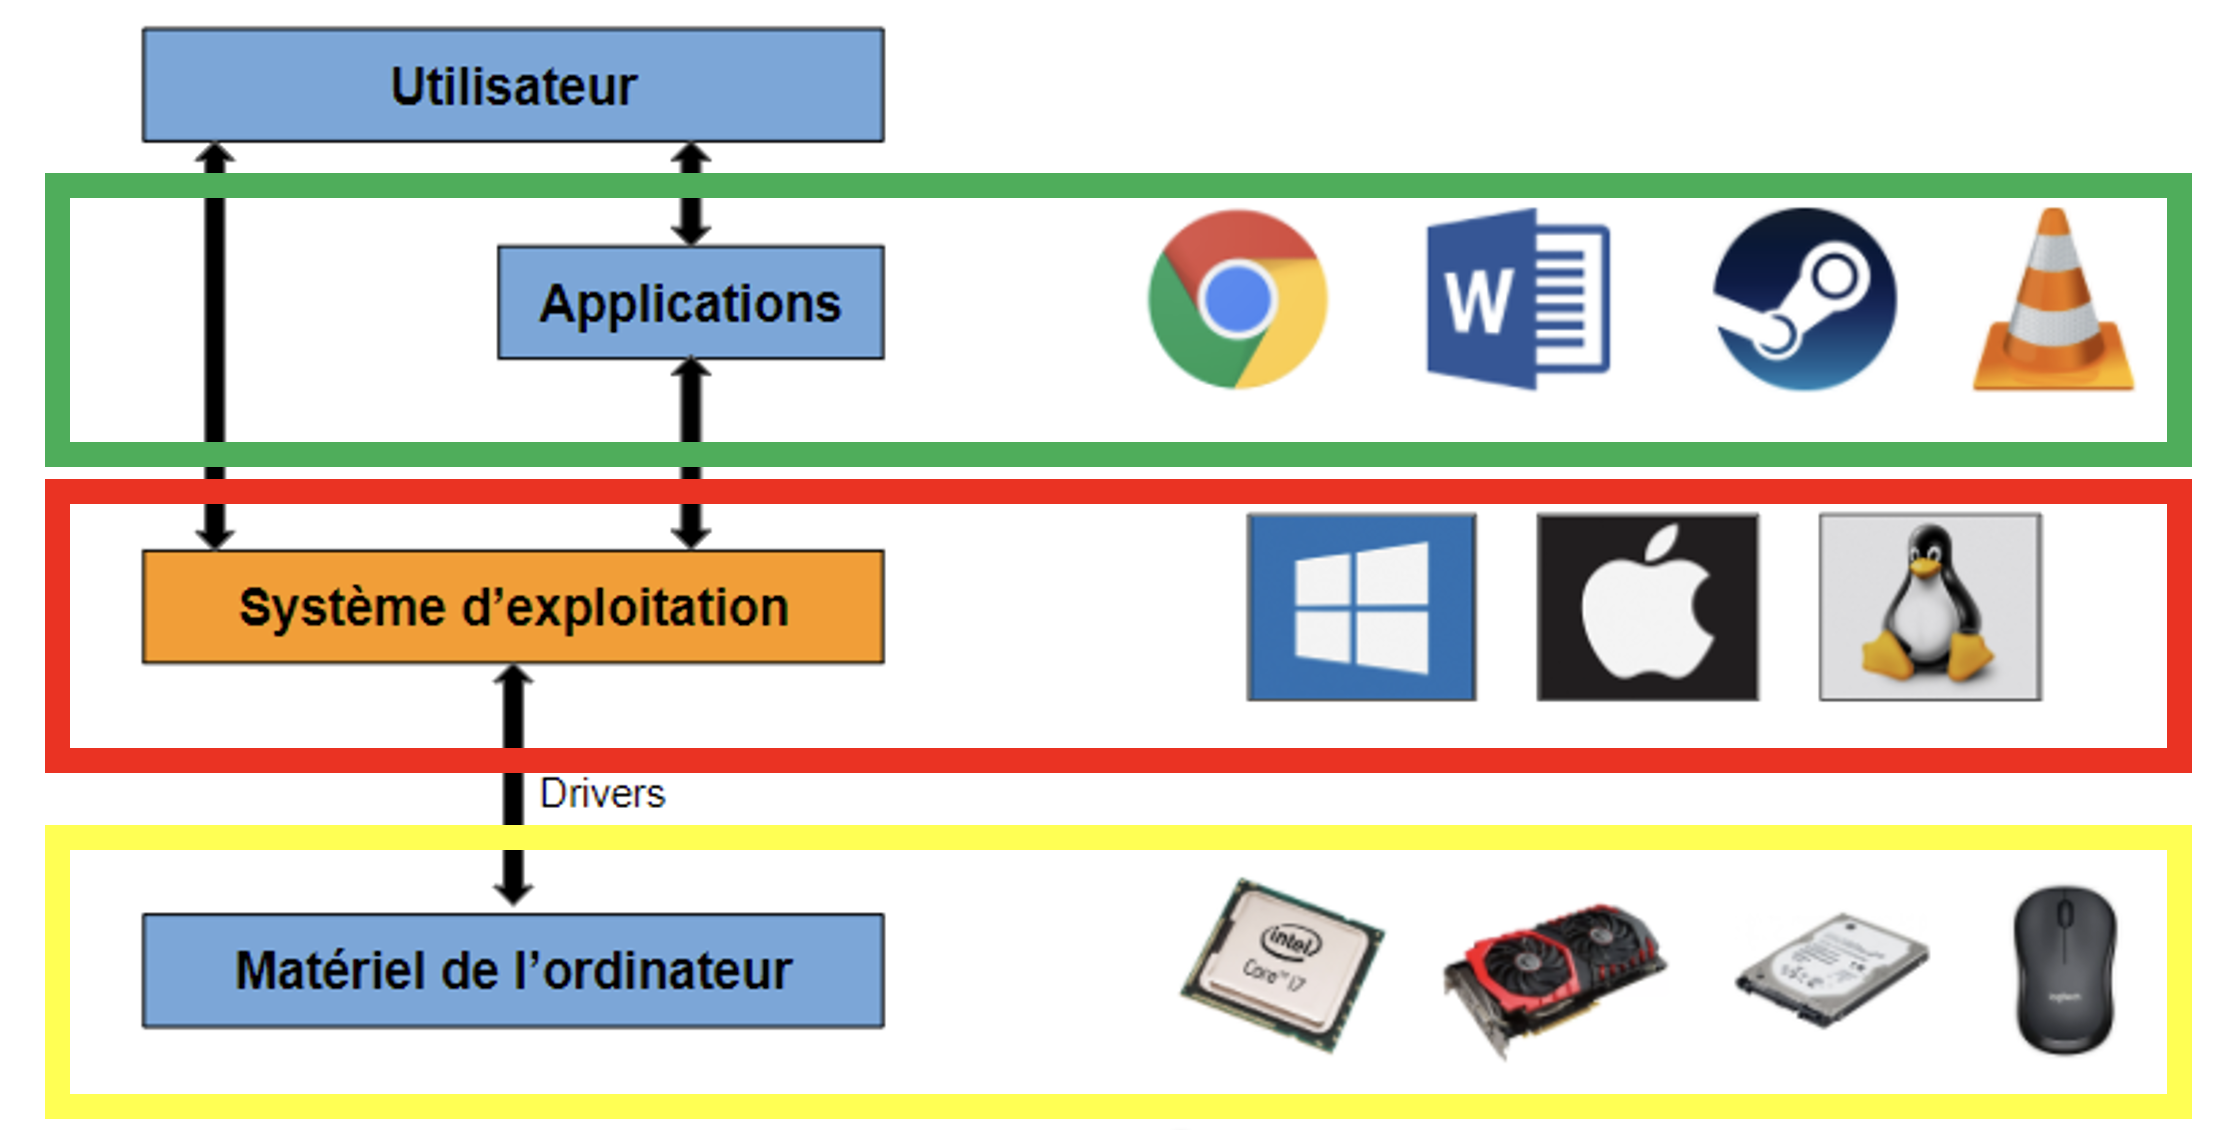
\includegraphics[width=0.7\textwidth]{001_OS.png}
	\end{figure}
	
	Dans le schéma ci-dessus on trouve:
	\begin{description}
		\item[\grnfrm{Dans le cadre vert:}] La "couche applicative" --- les programmes et applications qu'utilisent les utilisateurs finaux et que, cette année, nous avons commencé à apprendre à développer en Python;
		\item[\redfrm{Dans le cadre rouge:}] Un des objets de ce cours, la couche intermédiaire située entre le matériel et l'applicatif, l'OS ("Operating System") ou système d'exploitation en français;
		\item[\yelfrm{Et enfin dans le cadre jaune:}] Les composants matériels, physiques de l'ordinateur que l'on a étudiés en début d'année et qu'on représente habituellement dans le modèle de von Neumann -- et qui par lesquels nous allons commencer dans ce cours en étudiant les langages machine et assembleur.
	\end{description}
	

	Spécifiquement, dans cette thématique du cours, on va parcourir des éléments du schéma précédent et en "sortir" également un petit peu:
	\begin{itemize}
		\item Présentation des niveaux de langage les plus proches de la machine --- le langage machine et le langage assembleur;
		\item Pratique: visualisation de quelques opérations effectuées en langage assembleur (x86) et simulation quelques programmes simples;
		\item Introduction aux systèmes d'exploitation -- ce qu'ils sont, à quoi ils servent, pourquoi nos outils informatiques contemporains (ordinateurs, smartphones, tablettes, mais aussi voitures, télévisions, trains...) ne pourraient pas fonctionner sans;
		\item Pratique: exercices de lignes de commande en shell (interface système);
		\item Réseaux et internet --- introduction au modèle OSI;
		\item Pratique: exercices de configuration réseau dans le logiciel de simulation Filius.
	\end{itemize}

	\subsection{Comment réviser / préparer les contrôles?}
	
	Comme pour les autre chapitres de cours de NSI, les deux choses les plus importantes que vous devez acquérir pour être en mesure de bien réussir les contrôles sont:
	\begin{itemize}
		\item Connaître et comprendre les notions présentées dans le cours (et en particulier les définitions);
		\item Être capable de faire tous les exercices présents dans ce cours et également dans le cahier d'exercices qui l'accompagne.
	\end{itemize}
	 
	 Comme pour les chapitres précédents, chaque section de ce cours se termine par un encart (sur fond vert) intitulé "À Savoir \faExchange \ À Réviser" dans lequel je vous explique plus en détails ce qu'il y a à retenir de la section en question.
	 
	 En tout état de cause mon conseil principal pour les révisions est de prendre la version de ce cours et du cahier d'exercices qui ne contient \textit{\textbf{pas}} les solutions, vous exercer à faire les exercices qui sont dedans, puis vérifier les réponses dans la version qui contient les solutions.
	 
	 Bon courage!
	 
	 \pagebreak
	
	 \section{Les langages de bas niveau}
	 
	 \subsection{Un peu d'Histoire...}
	 On a vu en tout début de cours sur la programmation que les langages informatiques se distinguent (entre autres) par ce qu'on appelle leur "niveau": plus celui-ci est dit "bas" plus on est proche des objets physiques qui constituent la machine, plus au contraire il est "haut" plus on s'en éloigne pour arriver dans des vocables / syntaxes / grammaires compréhensibles par l'être humain --- par exemple le langage Python ou, plus élevé encore, le pseudo-code.
	 
	 \begin{figure}[H]
	 	\centering
	 	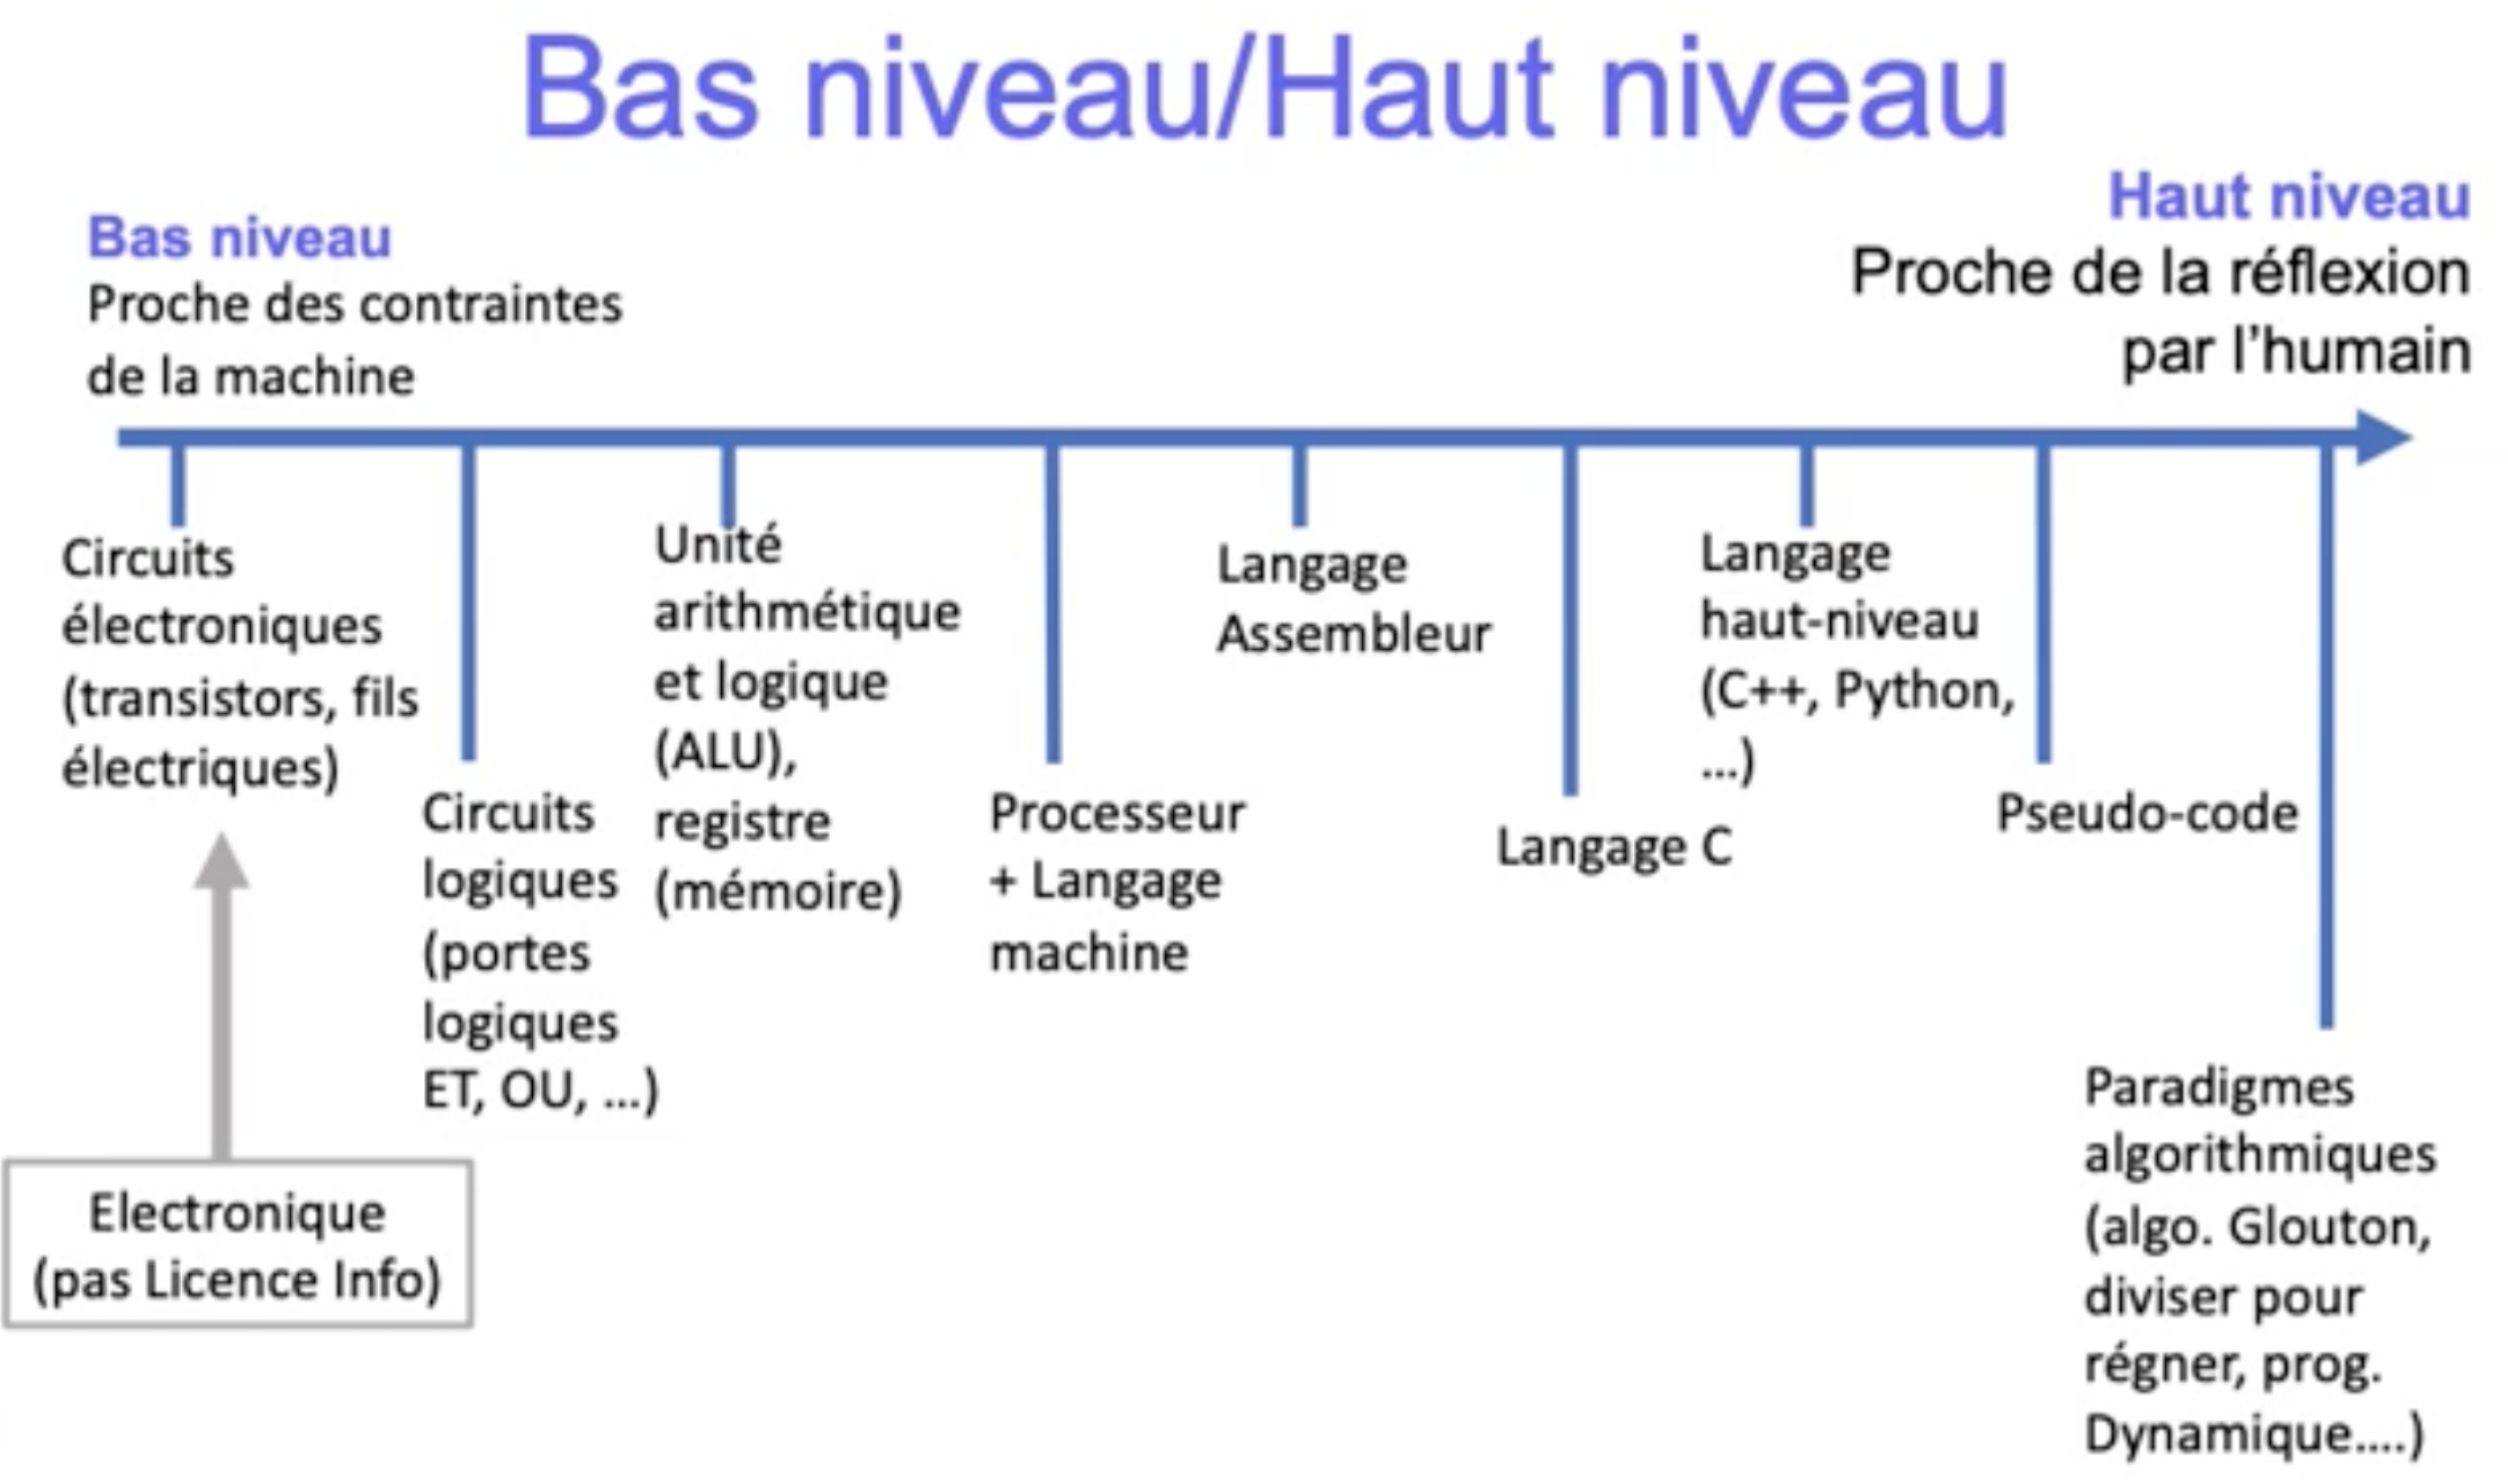
\includegraphics[width=\textwidth]{004_BasHautNiveau.png}
	 \end{figure}
	 
	 Aux origines de l'informatique, les "langages" n'existaient pas (les claviers, d'ailleurs, non plus): toute la programmation se faisait par la câblage manuel de la machine pour qu'elle réalise une tâche spécifique. Lorsqu'on souhaitait qu'elle en réalise une autre, le câblage devait être modifié, comme dans la photographie ci-dessous\footnote{Photographie du calculateur ENIAC prise en 1946, obtenue \href{https://lejournal.cnrs.fr/sites/default/files/styles/lightbox-hd/public/assets/images/1946_eniac_iv_72dpi.jpg?itok=Y1FhKfw_}{textsur le site du CNRS}.}. A l'époque, les rôles de concepteur, constructeur, programmeur, opérateur et utilisateur étaient donc confondus --- c'était un seul et même ingénieur qui faisait tout (ou, pour se référer au schéma ci-dessus, les tâches correspondant à la totalité des niveaux étaient réalisées par la même personne).

	 \begin{figure}[H]
	 	\centering
	 	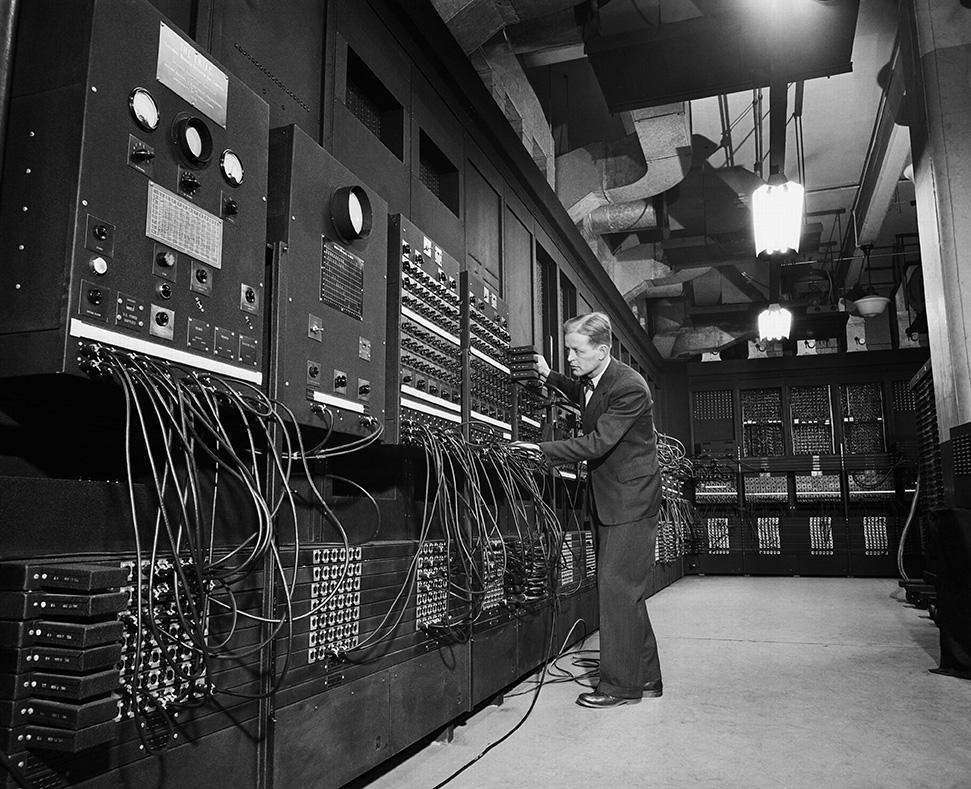
\includegraphics[width=\textwidth]{005_Eniac.jpg}
	 \end{figure}
	 
	 C'est dans les années 1950 et surtout 1960 avec l'utilisation de plus en plus généralisée des transistors que la nécessité de câbler les machines a progressivement disparu, leur miniaturisation a été engagée, et les langages pour communiquer avec les composants micro-électroniques sont nés.
	 
	 \MaQuest{Pourquoi la région de Californie où sont localisées la plupart des grandes entreprises de technologie est-elle nommée la Silicon Valley?} 
	 
	 \begin{MaReponse}
	 	C'est une bonne question quand on pense que le silicone est une forme de mastic ou de caoutchouc...
	 	
	 	\noindent
	 	\begin{minipage}{0.5\textwidth}
	 		\centering
	 		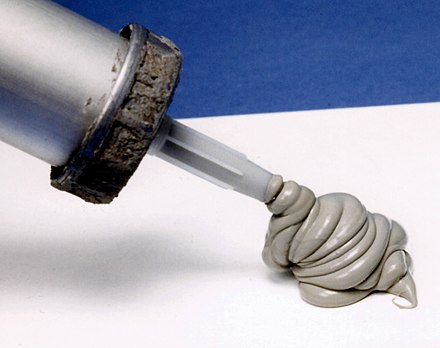
\includegraphics[width=0.8\linewidth]{006_Silicone1.jpg}
	 	\end{minipage}%
	 	\begin{minipage}{0.5\textwidth}
	 		\centering
	 		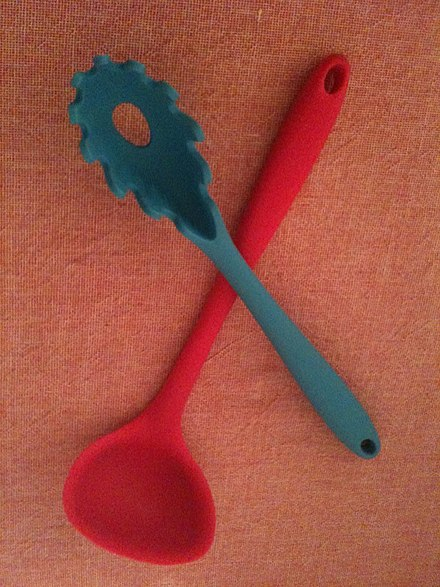
\includegraphics[width=0.5\linewidth]{007_Silicone2.jpeg}
	 	\end{minipage}
	 	
	 	C'est en fait simplement un problème de traduction: l'élément silicium, avec lequel on fabrique beaucoup de semi-conducteurs et notamment les transistors, se dit "\textit{silicon}" en anglais.
	\end{MaReponse}
	
	\begin{wrapfigure}{r}{0.\textwidth}
		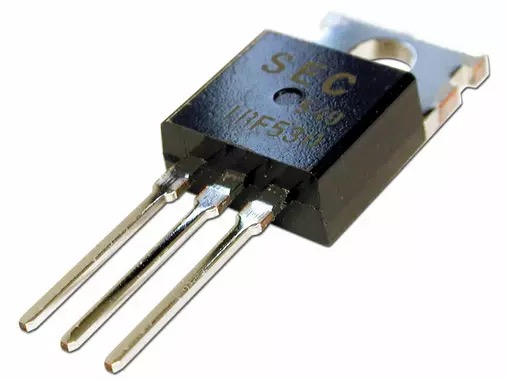
\includegraphics[scale=0.3]{009_Transistor.jpg}
	\end{wrapfigure}
	Pour faire simple, un transistor est un interrupteur (ayant donc deux positions, correspondant au 0 et au 1) qui est pilotable par un courant électrique: on peut donc connecter électriquement plusieurs transistors ensemble (pour former un circuit), les uns pilotant les autres, ce qui permet c'est de constituer dans un premier temps des portes logiques telles que celles que l'on a vues au chapitre sur les booléens (AND, OR, XOR...). Ces circuits prennent en entrée une ou plusieurs tensions électriques et en font ressortir une en fonction du câblage réalisé --- ce qui, logiquement, se traduit par un ou plusieurs bits en entrée et un bit unique en sortie (vous vous souvenez des tables de vérité qu'on avait étudiées? C'est exactement de cela que l'on parle ici).
	
	 \subsection{Quelle langue parle mon ordinateur?}

	On a vu plus haut le schéma ci-dessous qui illustre la position des systèmes d'exploitation -- entre le matériel et l'applicatif: on va s'intéresser dans ce chapitre à la partie basse de ce schéma.
	
	 \begin{figure}[H]
	 	\centering
	 	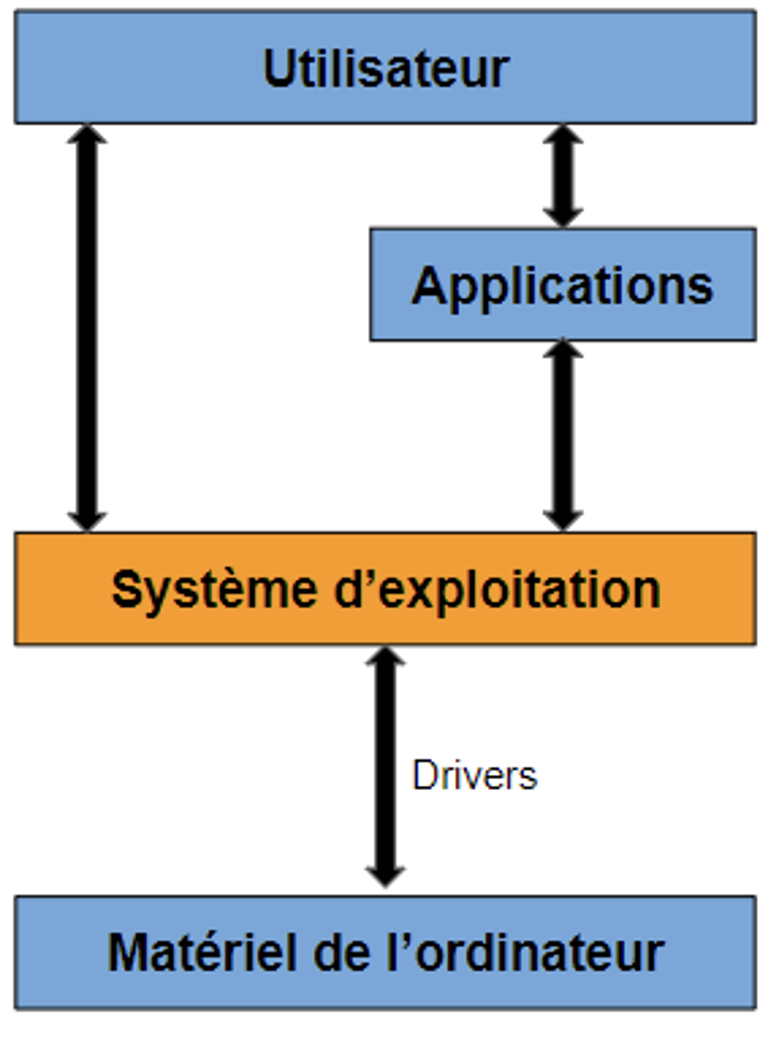
\includegraphics[width=0.3\textwidth]{003_CouchesOrdi.png}
	 \end{figure}
	 
	 \MaQuest{Mais avant de nous lancer dans cette histoire de langage, si on commençait par un petit rappel: quels sont les éléments principaux de l'architecture de von Neumann qu'on a vue en début d'année --- \textit{indice: il y en a 3...}?}
	 
	 	\begin{MaReponse} 
	 	
	 	\begin{figure}[H]
	 		\centering
	 		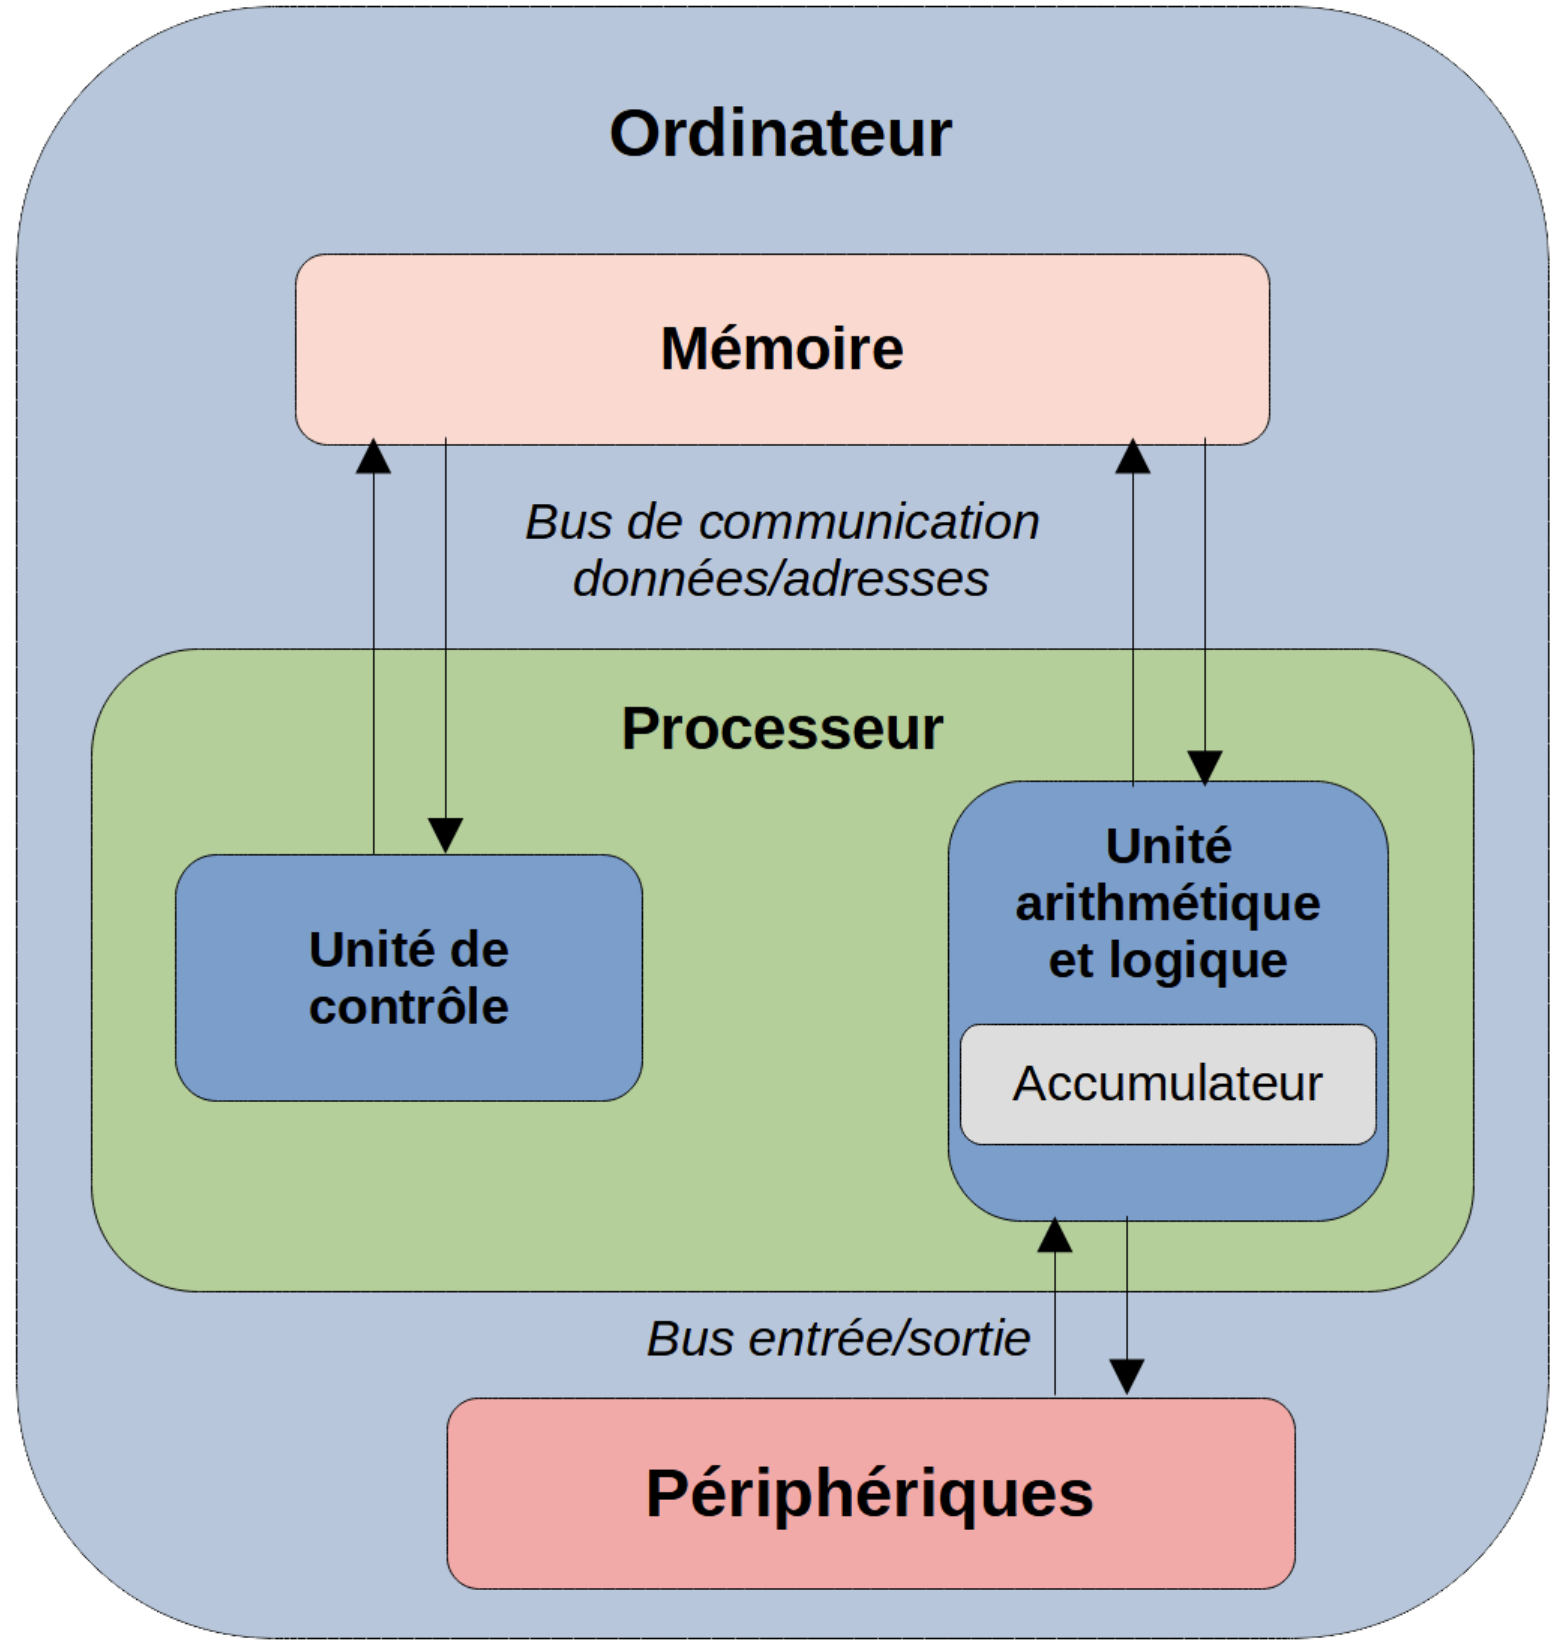
\includegraphics[width=0.5\textwidth]{002_VonNeumann.png}
	 	\end{figure}
	 	
	 	Ce modèle nous fournit une représentation simplifiée mais exacte de l'architecture matérielle d'un ordinateur (ou, plus généralement, de n'importe quel matériel qui s'appuie sur l'informatique). Les différents éléments qui le constituent ont les rôles suivants:
	 	
	 	\begin{description}
	 		\item[Unité Arithmétique et Logique:] elle effectue les opérations de base;
	 		\item[Unité de Contrôle:] elle assure le séquencement des opérations à effectuer;
	 		\item[Mémoire:] elle contient à la fois les données qui vont être utilisées et les programmes qui s'en chargeront et indiqueront à l'unité de contrôle quelles opérations vont être nécessaires. Elle se divise en deux parties:
	 		
	 		\begin{alphenum}
	 			\item La mémoire volatile, ou mémoire vive utilisée en cours d'exécution de programmes;
	 			\item La mémoire permanente qui contient les programmes et données que l'on va conserver sur l'appareil.
	 		\end{alphenum}
	 		
	 		\item[Périphériques:] ce sont des dispositifs d'entrée / sortie qui vont permettre de communiquer avec l'extérieur. Il y en a une multitude: clavier, imprimante, carte réseau, micro, enceinte, écran, souris,...
	 	\end{description}
	 	
	 \end{MaReponse}
	 
	 	 
	 L'enjeu de ce chapitre est de s'intéresser au langage que comprend le cerveau de notre ordinateur, son processeur: les "instructions machine".
	 
	 \begin{MaDef}{Instruction machine}
	 	Une \textbf{instruction machine} est une chaîne binaire composée principalement de deux parties:
	 	\begin{itemize}
	 		\item Le champ "code opération" qui indique au processeur le type de traitement à réaliser;
	 		\item Le champ "opérandes" indique la nature des données sur lesquelles l'opération désignée par le "code opération" doit être effectuée.
	 		
	 		\begin{figure}[H]
	 			\centering
	 			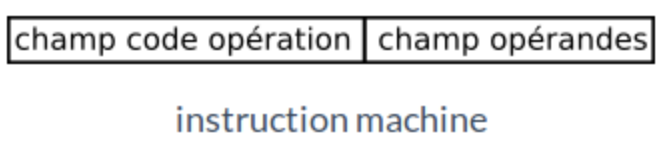
\includegraphics[width=0.5\textwidth]{008_InstrMach.png}
	 		\end{figure}
	 	\end{itemize}
	 \end{MaDef}
	 
	 Ces instructions machines sont donc des mots binaires qui, à l'instar des données qu'elles manipulent, sont stockées dans la mémoire de l'ordinateur, dans des cases mémoire possédant chacune une adresse (ces cases, selon l'architecture de la machine, peuvent être de 8, 16, 32, ou 64 bits). On peut se représenter cette mémoire comme une pile de cases contenant chacune un élément qui sera soit une instruction soit une donnée. 
	
	On peut imaginer par exemple dans une architecture en 32 bits l'instruction suivante: \texttt{11100011 10100000 0000010 00010000} où les deux premiers octets constitueraient le code opération (disons par exemple "copie") puis les deux suivants les adresses mémoires des informations à copier (source / cible).
	
	Un programme informatique deviendrait donc une suite de telles instructions --- par exemple, un programme extrêmement simple n'occupant que 9 cases mémoire pourrait s'écrire:
	
	\begin{Verbatim}
		11100011 10100000 00000000 00000100
		11100101 10001111 00000000 01101100
		11100011 10100000 00000000 00001000
		11100101 10001111 00000001 00011000
		11100101 10011111 00000000 01100000
		11100011 01010000 00000000 00001010
		00011010 00000000 00000000 00000010
		11100011 10100000 00000000 00001001
		11100101 10001111 00000001 00000100
	\end{Verbatim}
	 
	 Alors, me direz-vous, c'est bien gentil tout ça --- mais pas franchement clair... C'est ce qui nous amène au langage assembleur.
	 
	 \subsection{Langage assembleur}
	 
	 \subsubsection*{Pourquoi s'intéresser à cela?}
	
	Il n'est pas question ici de faire de vous des programmeurs en assembleur, ça n'aurait strictement aucun intérêt, même si c'est un métier qui existe et est vital dans bien des domaines --- le développement de compilateurs, le développement de pilotes (drivers), la programmation de certaines tâches sur des systèmes embarqués... Mais ce métier est extrêmement spécialisé, et si vous devez y venir ce ne sera que dans plusieurs années.
	
	L'intérêt de cette introduction est plutôt de vous ouvrir une fenêtre sur le fonctionnement interne des machines que l'on manipule depuis le début de l'année, vous faire comprendre ce que, en réalité, elles savent faire, et donc comment les programmes que vous concevez et réalisez en Python sont, dans la pratique, mis en œuvre par votre ordinateur.
	
	\subsubsection*{Les mnémoniques}
	
	 Le "code opération" dont on a parlé plus haut est nécessairement quelque chose d'immuable: il a dû être programmé dans le processeur à sa construction. Il y en a en fait relativement peu --- il peut s'agir de:
	 \begin{itemize}
	 	\item Opérations arithmétiques: addition, soustraction, multiplication...
	 	\item Transferts de données d'une "case" mémoire à une autre.
	 	\item Rupture de séquence (si l'on effectue une boucle par exemple, ou si on applique une condition et qu'en conséquence on ne va plus enchaîner les instructions dans l'ordre prévu).
	 	\item Opérateurs de comparaison.
	 \end{itemize}
	 
	 Ces opérations se traduisent en langage assembleur en ce que l'on appelle des "mnémoniques": des codes de trois lettres de long plus ou moins explicite correspondant exactement et de manière unique à une opération élémentaire que sait réaliser le processeur et qui donc sera traduit en le code opération correspondant. Par exemple:
	 \begin{description}
	 	\item[ADD] Addition de deux valeurs;
	 	\item[MOV] Copie d'une valeur d'une case mémoire vers une autre;
	 	\item[CMP] Compare deux valeurs;
	 	\item etc...
	 \end{description}
	 
	 Il va de soi, puisque ces opérations sont programmées "en dur" dans les processeurs des machines, que les langages assembleur sont spécifiques à l'architecture du processeur pour lesquels ils sont conçus. Cela signifie que chaque type de processeur a son propre langage assembleur, qui utilise des mnémoniques et des instructions adaptées aux capacités et à la structure interne de ce processeur particulier. Celui que nous utilisons ici est une version du langage "x86" adapté aux processeurs Intel et AMD équipant la plupart des PCs modernes.
	 
	 Vous constaterez qu'en passant d'un processeur à un autre, d'un simulateur à un autre même au sein de la famille des "x86" il existe de petites variations dans les mots utilisés et même dans la syntaxe (exemple avec la commande \texttt{STR} qui sert à stocker une valeur en mémoire et que dans différents systèmes on pourra trouver écrite \texttt{STO} ou \texttt{STA}). Il est cependant (comme c'est le cas pour \texttt{STR}) en général facile de deviner les transpositions de l'une à l'autre.
	 
	 \begin{MonAmp}{Fonctionnement d'un programme en assembleur}
	 	Un programme en assembleur est donc une succession d'instructions utilisant des mnémoniques --- il pourrait ressembler à:
	 	
	 	\begin{figure}[H]
	 		\centering
	 		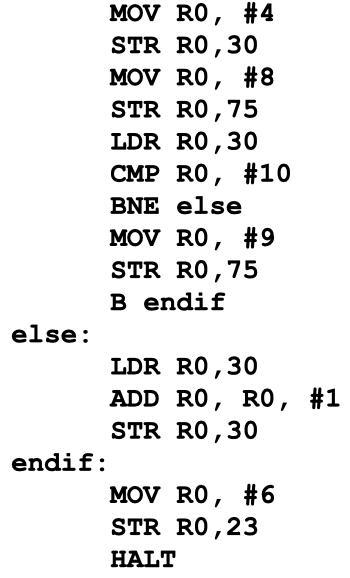
\includegraphics[width=0.3\textwidth]{010_Assembleur.png}
	 	\end{figure}
	 	
	 	C'est peu lisible --- mais ça l'est infiniment plus que l'étape suivante qui est une traduction de ce programme en instructions machine écrites en binaire.
	 \end{MonAmp}
	 
	 La chaine globale d'exécution d'un programme en langage informatique comme Python par exemple peut donc se représenter ainsi:
	 
	 \begin{figure}[H]
	 	\centering
	 	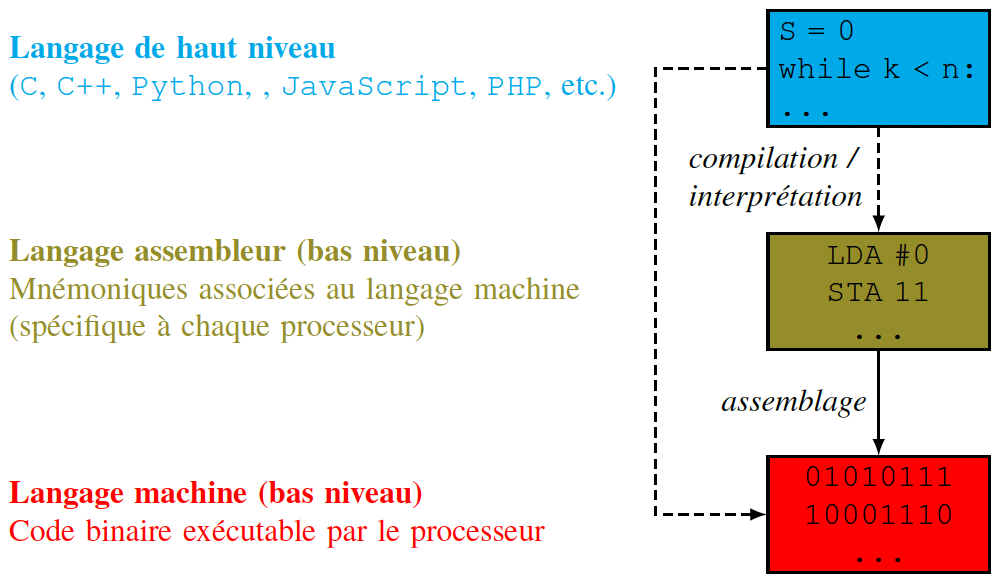
\includegraphics[width=0.8\textwidth]{011_Compilation.png}
	 \end{figure}
	 
	 \begin{MaDef}{Compilation, Interprétation, Assemblage}
	 	Voilà trois termes qui, sommairement, pourraient tous trois se définir comme des formes de "traduction" mais qui dans les faits, on devrait l'avoir compris d'après ce qui vient d'être présenté, sont tout à fait distincts les uns des autres:
	 	\begin{description}
	 		\item[Compilation] Processus qui consiste à convertir le code source écrit dans un langage de programmation de haut niveau (comme C ou Java) en code machine directement exécutable par le processeur d'un ordinateur. Ce processus est réalisé par un programme appelé compilateur. Le compilateur effectue cette conversion en une seule fois, générant un fichier exécutable que l'on peut lancer indépendamment du compilateur.
	 		\item[Interprétation] L'interprétation est une méthode d'exécution de programmes où le code source est exécuté directement, instruction par instruction, par un autre programme appelé interpréteur. Contrairement à la compilation, l'interprétation ne produit pas de fichier exécutable permanent; l'interpréteur lit le code source, le traduit en instructions machine au fur et à mesure et exécute ces instructions immédiatement. Cela permet une plus grande flexibilité et facilité de débogage, mais peut réduire la vitesse d'exécution comparée à un programme compilé. C'est ce que nous utilisons avec notre code Python dans le cadre de ce cours.
	 		\item[Assemblage] L'assemblage est le processus de conversion du code source écrit en langage assembleur (un langage de bas niveau proche du langage machine mais légèrement abstrait avec des mnémoniques) en code machine binaire. Ce processus est effectué par un programme appelé assembleur. Le langage assembleur permet aux programmeurs de contrôler plus directement le matériel et est souvent utilisé pour des tâches nécessitant une optimisation de performance ou pour interagir directement avec le matériel de l'ordinateur.
	 	\end{description}
	 	
	 	On notera ici une différence importante entre les deux premières notions qui consistent en une interprétation d'un langage pour passer à des instructions machine et nécessite de l'intelligence (une seule instruction Python par exemple pouvant être traduite en plusieurs instructions machine) et la troisième qui n'est en fait qu'une traduction "mot à mot".
	 \end{MaDef}
	 
	 \subsubsection*{Mise en pratique sur un simulateur}
	 
	 Nous allons dans cette section utiliser \href{https://www.peterhigginson.co.uk/AQA}{le simulateur mis en ligne par Peter Higginson}.
	 
	 \begin{MonExo}[Premières instructions en assembleur]
	 	\textbf{Cet exercice est à réaliser dans un document texte (format de votre choix) et à me soumettre soit par mail soit dans mon casier sur l'ENT.}
	 	\begin{alphenum}
	 		\item Dans un moteur de recherche, rechercher "simulateur aqa peter higginson" et vous rendre sur la page correspondante.
	 		\item Effectuez une par une les opérations suivantes dans le simulateur (en utilisant le bouton \texttt{STEP}) et expliquez ce qu'elles font:
	 		\begin{alphenum}
	 			\item \texttt{MOV R3,\#78}
	 			\item \texttt{STR R3,50}
	 			\item \texttt{LDR R1,50}
	 			\item \texttt{ADD R2,R1,\#30}
	 			\item \texttt{ADD R0,R1,R2}
	 		\end{alphenum}
	 		\item Sur la base de vos essais ci-dessus, quelle est la différence entre \texttt{50} et \texttt{\#50}?
	 		\item Peut-on réaliser les deux premières opérations ci-dessus en une seule fois (faites l'essai!)?
	 		\item En quoi selon vous \texttt{MOV}, \texttt{LDR} et \texttt{STR} sont-ils des mnémoniques --- à quels mots (en anglais) font-ils référence?
	 	\end{alphenum}
	 \end{MonExo}
	 
	 \begin{MonExo}[Etudions à présent un programme complet]
	 	Soit le programme suivant:
	 	\begin{minted}[linenos]{text}
INP R0,2
INP R1,2
CMP R1,R0
BGT HIGHER
OUT R0,4
B DONE
HIGHER:
OUT R1,4
DONE:
HALT
	 	\end{minted}
	 	Copiez le dans le simulateur et lancez-le plusieurs fois.
	 	\begin{alphenum}
	 		\item Que fait ce programme --- quelle serait sa docstring si vous deviez la rédiger?
	 		\item A quoi servent les mnémoniques \texttt{INP} et \texttt{OUT}?
	 		\item Et \texttt{B} / \texttt{BGT}?
	 		\item A quoi sert selon vous le premier registre (intitulé \texttt{PC})?
	 		\item Modifiez-le pour qu'il ne prenne qu'un nombre en entrée et renvoie le plus petit entre celui-ci et la valeur stockée en mémoire à la case 50 (indice: vous aurez besoin de consulter les mnémoniques utilisés à l'exercice précédent).
	 	\end{alphenum}
	 \end{MonExo}
	 
	 \begin{MonExo}[Etudions la correspondance avec Python]
	 	Soit le code Python suivant:
	 	\MonPython{001_SimAss.py}
	 	
	 	Son interprétation en assembleur est la suivante:
	 	\begin{minted}[linenos]{text}
MOV R0, #4
STR R0,30
MOV R0, #8
STR R0,75
LDR R0,30
CMP R0, #10
BNE else
MOV R0, #9
STR R0,75
B endif
else:
LDR R0,30
ADD R0, R0, #1
STR R0,30
endif:
MOV R0, #6
STR R0,23
HALT
	 	\end{minted}
	 	
		\begin{alphenum}
			\item Analysez la correspondance entre les deux programmes: dressez un tableau faisant correspondre chaque ligne Python avec celle(s) en assembleur.
			\item À quoi correspondent les adresses mémoires 23, 75 et 30?
		\end{alphenum}
		
		N'hésitez pas à utiliser le simulateur pour vous aider!
	 \end{MonExo}
	 
 	\begin{MonRet}
	 	Ce qu'il faut retenir de cette section sur le langage assembleur est:
	 	\begin{itemize}
	 		\item Comprendre et pouvoir sommairement expliquer l'évolution historique de l'informatique qui a amené à l'avènement des langages informatiques;
	 		\item Se remémorer le modèle de von Neumann;
	 		\item Comprendre et pouvoir expliquer les notions de langage machine et langage assembleur;
	 		\item Comprendre et pouvoir expliquer les différents niveaux de langage informatique et les processus de passage de l'un à l'autre (compilation...);
	 		\item Sans connaître par cœur les mnémoniques que nous avons utilisés ici, être capable de réaliser des exercices du type des trois précédents --- et notamment le dernier dans lequel il s'agit de lire du code assembleur et de le relier à son code Python correspondant.
	 	\end{itemize}
		\end{MonRet}
	 
\end{document}
	 	
	\subsection{Introduction}

	\begin{MaVid}
		\href{https://www.youtube.com/watch?v=SpCP2oaCx8A&feature=youtu.be}{Vidéo Youtube de l'INRIA} présentant les rôles principaux d'un système d'exploitation.
	\end{MaVid}
	
	Comme on l'a vu dans cette vidéo 
	
	
		

\end{document}

%Eléments manquants:
